\begin{solution}
\begin{enumerate}
\item {[8 points]} Suppose $u,v \in V$, so that $u(0)-u'(0)=v(0)-v'(0)=u(1)=v(1)=0.$
      Integrating by parts twice yields
\begin{eqnarray*}
 (Lu,v) &=& \int_0^1 -u''(x)v(x) \,dx \\[0.5em]
        &=& \Big[ -u'(x)v(x)\Big]_0^1 + \int_0^1 u'(x)v'(x)\,dx, \\[.5em]
        &=& -u'(1)v(1)+u'(0)v(0) + \int_0^1 u'(x)v'(x)\,dx,\\[.5em]
        &=& -u'(1)v(1)+u'(0)v(0) + \Big[ u(x)v'(x)\Big]_0^1 - \int_0^1 u(x)v''(x)\,dx\\[.5em]
        &=& -u'(1)v(1)+u'(0)v(0) + u(1)v'(1)-u(0)v'(0) + (u,Lv)\\[.5em]
        &=& (u,Lv).
\end{eqnarray*}
In the last step, two boundary terms are zero because $u(1)=v(1)=0$.
For the other boundary term, note that $v(0)-v'(0)=0$ implies $v(0)=v'(0)$,
so $u'(0)v(0) - u(0)v'(0) = u'(0)v(0) - u(0)v(0) = -(u(0)-u'(0))v(0) = 0$
since $u(0)-u'(0)=0$.  Hence $(Lu,v) = (u,Lv)$ for all $u,v \in V$ and so $L$ is symmetric.
\\
\item {[8 points]} Zero is \emph{not} an eigenvalue of $L$.  To see this, 
      we seek a nonzero solution $\psi\in V$ to $L\psi = 0 \psi$, i.e., $-\psi''(x) = 0$.
      The general solution of $-\psi''(x) = 0$ is $\psi(x) = A x + B$ where $A$ and $B$ are constants.
      The right boundary condition $\psi(1)=0$ implies that 
       \[ 0 = \psi(1) = A + B,\]
      hence $A = -B$.  The left boundary condition implies
       \[ 0 = \psi(0) - \psi'(0) = B - A,\]
      hence $A=B$.  The only solution which satisfies both of these conditions is hence
      $A=B=0$, so $\psi(x) = 0$ is the only solution 
      of $L\psi = 0$.
      Thus zero is not an eigenvalue of $L$.
\\
\item {[8 points]} Suppose $u\in V$, so that $u(0)-u'(0)=u(1)=0.$ Then, integrating by parts gives
\begin{eqnarray*}
 (Lu,u) &=& \int_0^1 -u''(x)u(x) \,dx \\[0.5em]
        &=& \Big[ -u'(x)u(x)\Big]_0^1 + \int_0^1  u'(x)u'(x)\,dx, \\[.5em]
        &=& -u'(1)u(1)+u'(0)u(0) + \int_0^1 (u'(x))^2\,dx.\\[.5em]
\end{eqnarray*}
Now, $(u'(x))^2\ge0$ for all $x\in[0,1]$ and so $\int_0^1 (u'(x))^2\,dx\ge0$. Moreover, since  $u(1)=0$ we have that $-u'(1)u(1)=0$ and since $u(0)-u'(0)=0$ we can say that $u(0)=u'(0)$ from which it follows that $u'(0)u(0)=(u(0))^2\ge0$. Therefore, $\ip{Lu,u}\ge0$ for all $u\in V$.

If $\lambda$ is an eigenvalue of $L$ then, since $L$ is a symmetric linear operator, $\lambda\in\R$ and there exist nonzero $\psi\in V$ which are such that $L\psi=\lambda\psi$ and hence
\[
 \lambda(\psi,\psi) = ( \lambda\psi,\psi)= ( L\psi,\psi).
\]
The fact that $\ip{Lu,u}\ge0$ for all $u\in V$ then means that
\[
 \lambda = {( L\psi,\psi) \over (\psi,\psi)}\ge0
\]
since $(\psi,\psi)>0$ by the definition of the inner product because $\psi$ is a nonzero function. However, in part (b) we had showed that zero is not an eigenvalue of $L$ and so we can conclude that $\lambda >0$ for all eigenvalues $\lambda$ of $L$.
\\
\item {[8 points]} We now know that all eigenvalues $\lambda$ of $L$ are positive and so the general solution of $L\psi = \lambda \psi$, i.e. $-\psi'' = \lambda \psi$, has the form
      \[
\psi(x) = A \sin(\sqrt{\lambda} x) + B \cos(\sqrt{\lambda} x)
\]
 where $A$ and $B$ are constants. The left boundary condition gives
      \[
0 = \psi(0) - \psi'(0) = A \sin(0) + B \cos(0)- A \sqrt{\lambda} \cos(0)+ B \sqrt{\lambda} \sin(0)= B - A \sqrt{\lambda},
\]
      hence $B = A \sqrt{\lambda}$.
      The right boundary condition gives
      \[
0 = \psi(1) = A \sin(\sqrt{\lambda}) + B \cos(\sqrt{\lambda}).
\]
      Substituting the left boundary condition into this last formula, we find
       \[ 
0 = A \sin(\sqrt{\lambda}) + A \sqrt{\lambda} \cos(\sqrt{\lambda}).
\]
Since we need $A\ne 0$ in order for $\psi\ne0$, this equation implies that
       \[ 
\sqrt{\lambda} = - {\sin(\sqrt{\lambda}) \over \cos(\sqrt{\lambda})}
                         = -\tan(\sqrt{\lambda}).
\]
Therefore, the eigenfunctions of $L$ have the form
\[
\psi(x) = A(\sin(\sqrt{\lambda} x) + \sqrt{\lambda}\cos(\sqrt{\lambda} x)),\, A\ne0
\]
where the eigenvalues $\lambda$ are the positive numbers which are such that
\[
\sqrt{\lambda} = -\tan(\sqrt{\lambda}).
\]
\\
\item {[8 points]} The plot is shown below.

\begin{center}
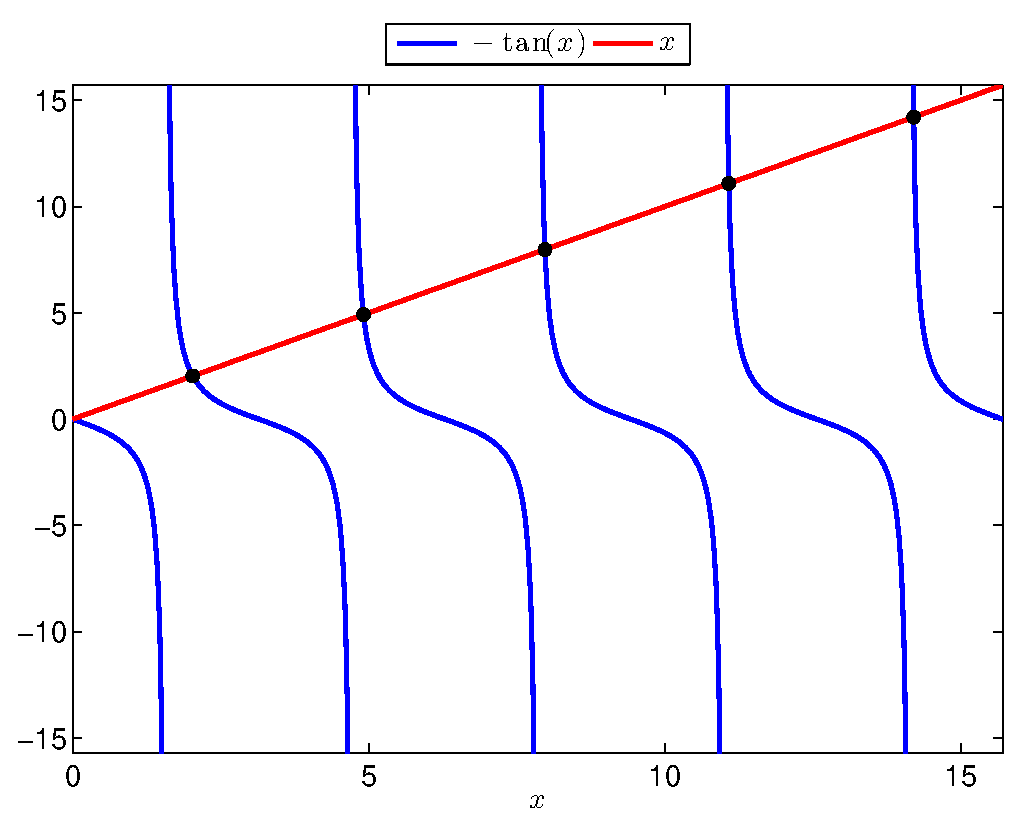
\includegraphics[scale=0.7]{eigroot}
\end{center}

From the plot we can see that there are 5 points where $g(x)$ and $h(x)$ intersect for $x\in(0,5\pi]$. Hence, since the eigenvalues $\lambda$ of $L$ are the positive numbers which are such that $g(\sqrt{\lambda})=h(\sqrt{\lambda})$, $L$ has five eigenvalues $\lambda$ which are such that $\sqrt{\lambda}\le 5\pi$.

The code used to produce the plot is below.

\lstinputlisting{HW24e.m}

The  function \verb|bisect| used in the above code is below.

\lstinputlisting{bisect.m}

\end{enumerate} 
\end{solution}